\section{Experiments}

\subsection{Experimental Setting}

The controlled environment isolates the effect of redundancy and candidate-set
size. It fixes a budget of four contexts and uses 16 candidates in the
redundancy study; the candidate-scaling study varies the pool size over
$K=4,8,16,32,64$ at duplicate ratio $.50$. Candidate value is generated from
a frozen subset-capable predictor, and Standalone Utility, the cached-only
router, and R-MUR use matched encoder and head capacity. All controlled
results are averaged over five seeds. The standalone oracle ranks candidates
by the true standalone marginal and keeps that order fixed. The sequential
oracle recomputes true marginals after every selection. The gap between these
two policies defines structural headroom.

The real-data study uses six standard traffic benchmarks: METR-LA, PEMS-BAY,
PEMS03, PEMS04, PEMS07, and PEMS08. The predictor is trained before routing
and kept fixed; it accepts arbitrary candidate subsets. For each dataset,
candidate pools are constructed from the training segment, the history length
is 12, the forecast horizon is 12, the candidate count is 16, and the context
budget is four. The primary comparison uses three seeds. The multi-target study
fixes 32 evenly spaced target sensors per dataset and constructs a separate
candidate pool for each target from the training split. We report the
anchor-only predictor, pooling all candidates, relevance ranking, maximum
marginal relevance, Standalone Utility, the cached-only router, R-MUR, the
standalone oracle, and the sequential oracle. Unless stated otherwise, R-MUR
uses a shortlist of four candidates and the ranking-calibrated objective of
Eq.~\eqref{eq:loss}.

Two further protocols test the scope of the conclusions. The strong-backbone
study replaces the ridge expert with a subset-capable spatio-temporal
transformer, keeps every other component of the protocol identical, fixes 16
targets per dataset and uses three seeds; the shortlist size is swept over
$q\in\{2,4,8,16\}$ and the number of expert evaluations per decision is
recorded. The second-family study re-instantiates the same router on
demonstration selection for a frozen in-context classifier over five public
image benchmarks, with the same candidate count, budget, shortlist sizes and
response-feature semantics, replacing the forecast vector by the classifier's
class logits.

\subsection{Structural Value of State-Conditioned Selection}

In the controlled redundancy study, structural headroom grows monotonically
with the duplicate ratio. Table~\ref{tab:redundancy} reports the oracle ladder.
At zero redundancy the standalone and sequential oracles coincide. As
redundancy increases, the gap reaches .286. At duplicate ratios .50 and .75,
the learned router exceeds the standalone oracle even though that oracle uses
the true standalone utilities. The gain therefore comes from re-evaluating
candidate value after the selected state changes, not from a better standalone
score.

% Controlled-study values: KBS_MUR/results/raw/R070_oracle_ladder_k16_b4_rgrid_s5_20260919_1540/aggregate.json
\begin{table}[t]
\centering
\small
\caption{Controlled redundancy study at $K=16$ and budget four. Gains are
loss reductions relative to the anchor-only predictor; results are averaged
over five seeds.}
\label{tab:redundancy}
\resizebox{\linewidth}{!}{%
\begin{tabular}{lrrrr}
\toprule
Duplicate ratio & Standalone oracle & R-MUR & Sequential oracle & Structural headroom\\
\midrule
0    & .6880 $\pm$ .0077 & .6636 $\pm$ .0101 & .6880 $\pm$ .0077 & .0000\\
.25  & .5161 $\pm$ .0054 & .5027 $\pm$ .0105 & .5813 $\pm$ .0064 & .1121\\
.50  & .3512 $\pm$ .0028 & .3652 $\pm$ .0030 & .4471 $\pm$ .0041 & .2145\\
.75  & .1771 $\pm$ .0019 & .2085 $\pm$ .0049 & .2481 $\pm$ .0035 & .2859\\
\bottomrule
\end{tabular}}
\end{table}

The same structural effect appears on real benchmarks. Over six datasets, 32
fixed targets per dataset, and three seeds, every one of the 576 target-seed
evaluations has positive structural headroom (minimum $.0101$).
Table~\ref{tab:headroom-real} summarizes the distribution over cells. The
positive fraction is one for every dataset, and the mean headroom ranges from
$.076$ to $.119$. State conditioning therefore creates measurable decision value
across targets rather than at a single sensor.

% Real-data headroom: results/derived/R134_six_dataset_matrix/headroom.json
\begin{table}[t]
\centering
\small
\caption{Real-data structural headroom over 32 fixed targets per dataset and
three seeds (96 cells per dataset, 576 in total). Every cell is positive; the
minimum across all datasets is $.0101$.}
\label{tab:headroom-real}
\begin{tabular}{lrrr}
\toprule
Dataset & Mean headroom & Median headroom & Positive fraction\\
\midrule
METR-LA & .0959 & .0844 & 1.000\\
PEMS-BAY & .1156 & .1204 & 1.000\\
PEMS03 & .1189 & .1077 & 1.000\\
PEMS04 & .0834 & .0725 & 1.000\\
PEMS07 & .0892 & .0835 & 1.000\\
PEMS08 & .0760 & .0729 & 1.000\\
\bottomrule
\end{tabular}
\end{table}

\subsection{Multi-Target R-MUR Benchmark}

We next evaluate learned routing under the six-dataset protocol. The
cached-only router first forms a shortlist of four candidates, and R-MUR
reranks that shortlist with compact predictor-response summaries. The
response-aware model is trained with marginal-utility regression and the
gap-weighted pairwise objective. Table~\ref{tab:deployable} compares
deployable selection policies, including the trivial pool-everything policy,
which is the strongest competitor on five of the six datasets (on PEMS-BAY the
cached-only router and the static-utility model edge past it).
R-MUR has the best average
rank ($1.33$ against $2.00$), leads every specialised policy on all six
benchmarks, and is \emph{significantly} ahead of the best competitor on three of the
six under target-level paired intervals (METR-LA $+.0067$ $[+.0041,+.0094]$,
PEMS-BAY $+.0303$ $[+.0203,+.0427]$, PEMS07 $+.0041$ $[+.0015,+.0070]$). It is
unresolved on two more (PEMS03 $+.0013$ $[-.0004,+.0030]$, PEMS04 $-.0008$
$[-.0050,+.0025]$) and significantly \emph{below} pooling on PEMS08 ($-.0026$
$[-.0042,-.0010]$). Relevance
and maximum marginal relevance are harmful on four of the six datasets, showing
that similarity and diversity do not reliably represent predictive utility;
neither ever beats pooling.

% Values in this table are taken from results/derived/R134_six_dataset_matrix/six_dataset_matrix.json
% (32 targets, three seeds, 96 cells per dataset); average ranks are computed over the six rows below.
% Paired target-level bootstrap intervals: results/derived/R146_six_dataset_paired/paired.json
\begin{table}[t]
\centering
\small
\caption{Deployable selection methods, including the trivial pool-everything
policy, the strongest competitor on five of the six datasets. Values are
prediction gains
averaged over 32 fixed targets per dataset; the final column is the average
rank across the six datasets.}
\label{tab:deployable}
\resizebox{\linewidth}{!}{%
\begin{tabular}{lrrrrrrr}
\toprule
Method & METR-LA & PEMS-BAY & PEMS03 & PEMS04 & PEMS07 & PEMS08 & Avg. rank\\
\midrule
Relevance (kNN) & -.0165 & -.0199 & -.0191 & +.0071 & -.0155 & +.0074 & 5.67\\
MMR & -.0180 & -.0249 & -.0102 & +.0098 & -.0085 & +.0075 & 5.33\\
Standalone Utility & +.0024 & +.0272 & +.0149 & +.0248 & +.0152 & +.0246 & 3.67\\
Cached-only router & +.0042 & +.0284 & +.0154 & +.0250 & +.0150 & +.0246 & 3.00\\
Pool all 16 & +.0080 & +.0254 & +.0256 & +.0365 & +.0242 & +.0359 & 2.00\\
R-MUR (ours) & \textbf{+.0146} & \textbf{+.0557} & \textbf{+.0269} & \textbf{+.0357} & \textbf{+.0284} & \textbf{+.0333} & \textbf{1.33}\\
\bottomrule
\end{tabular}}
\end{table}

Table~\ref{tab:consistency} reports the multi-target comparison. R-MUR
improves over Standalone Utility and over the cached-only router on every
dataset. Five datasets show positive target fractions of 94--100\%. METR-LA
shows the widest target-level variation, with 75\% of targets positive and
81--84\% exceeding the two deployable baselines. The response-aware stage uses
predictor evaluations for only one quarter of the candidate pool.

\begin{table}[t]
\centering
\small
\caption{Multi-target consistency of R-MUR. Differences and positive-target
fractions are computed over 32 fixed targets per dataset. Oracle recovery is
the pooled ratio of R-MUR gain to sequential-oracle gain.}
% Generated values: KBS_MUR/results/derived/R080b_hierarchical_summary/summary.json
% Delta columns are hierarchical bootstrap means (targets resampled, then runs within target).
\label{tab:consistency}
\resizebox{\linewidth}{!}{%
\begin{tabular}{lrrrrrr}
\toprule
Dataset & $\Delta$ vs Static & $\Delta$ vs Cached & Positive targets & $>$ Static & $>$ Cached & Oracle recovery\\
\midrule
METR-LA & .0123 & .0104 & .812 & .969 & .969 & .099\\
PEMS-BAY & .0285 & .0272 & .938 & 1.000 & .969 & .309\\
PEMS03 & .0121 & .0115 & 1.000 & 1.000 & 1.000 & .447\\
PEMS04 & .0109 & .0107 & 1.000 & .969 & .969 & .534\\
PEMS07 & .0132 & .0134 & 1.000 & 1.000 & 1.000 & .456\\
PEMS08 & .0088 & .0087 & 1.000 & .969 & .969 & .516\\
\bottomrule
\end{tabular}}
\end{table}

The two contrasts test different components of the method. Improvement over
Standalone Utility shows that state-conditioned marginal utility contains
decision information absent from a fixed candidate score. Improvement over
the cached-only router shows that predictor-response information and ranking
calibration add value beyond a state-conditioned score built from cached
representations alone.

\begin{figure*}[t]
  \centering
  
\includegraphics[width=0.98\textwidth]{figures/fig3_multitarget_delta.pdf}
  \caption{Target-level difference between R-MUR and Standalone Utility over
  32 fixed targets per dataset. Five datasets are positive on 94--100\% of
  targets; METR-LA shows wider target variation.}
  \label{fig:target-delta}
\end{figure*}

Among the fourteen methods compared across the six benchmarks (the detailed
two-dataset matrix below reports eleven of them) is a DELIFT-style rule (ICLR 2025) that
combines submodular coverage with k-means representatives, implemented here as
greedy facility location over an over-segmented pool of cluster medoids. It is
significantly below pooling on all six datasets ($-.0196$ $[-.0241,-.0155]$ on
METR-LA, $-.0212$ $[-.0297,-.0128]$ on PEMS-BAY, and between $-.018$ and
$-.023$ elsewhere), so adding the most recent member of the submodular family
does not change the verdict: the strongest competitor is still the trivial
policy of using every candidate, and on every dataset the best non-trivial rule
is greedy mutual information.

\paragraph{Where a method change could still pay.} Every remaining loss in this
regime has one shape: the router wins on average while losing on a substantial
minority of episodes, and on PEMS08 it loses on average. The per-episode gains
all six deployments record put a ceiling on what any episode-level confidence
gate could recover: taking the better of routing and pooling episode by episode
would add $+.0148$ to $+.0778$ over pooling, three to seven times the router's
own advantage, and would convert the PEMS08 loss into a gain. The router loses
on $39$--$52\%$ of episodes, so the loss is a near-even split rather than a few
outliers a safety rule could excise. We then tested whether that headroom is reachable, and it is not.
Four signals available at decision time were recorded for every episode --- the
cached screen's top-two margin, the utility model's top-two margin, its top
score, and the prediction-change norm of the candidate it picked --- and each was
scored for predicting whether the router beats pooling on that episode. All
twelve dataset-by-signal AUCs lie in $[.481,.521]$: the router's own confidence
carries no information about when it is wrong, and the best held-out gate adds
at most $+.0030$ over pooling against a ceiling of $.013$ to $.048$. This is what
\cref{prop:suff} predicts rather than a defect of this router --- the
identifiable term is the anchor's residual, a strong anchor has absorbed its
systematic part, and what remains is noise, which no function of the same
absorbed signal can anticipate. The remaining loss is therefore not a tuning,
head-design or gating problem: the estimation error is present and
unobservable.

\subsection{The standard selection toolkit is harmful when utility is estimable}
\label{sec:ridge-matrix}

The ridge protocol is the regime in which context selection has realizable
value, because the expert's residual is systematic and therefore predictable.
\Cref{tab:ridge-matrix} evaluates the full competitor set on the same 32
targets and three seeds. Two results stand out.

First, \emph{the default heuristics are significantly harmful on both datasets}:
relevance ranking is $.0165$ below the anchor-only predictor on METR-LA and
$.0199$ below on PEMS-BAY, MMR is $.0180$ and $.0249$ below, and on METR-LA
DPP, k-center, facility location, k-means representatives, random subsets and
even greedy mutual information are harmful as well, each with a target-level
interval entirely below zero. Selecting correlated or diverse candidates by a
proxy score injects noise that the predictor propagates; the oracles show that
a great deal of value exists ($+.133$/$+.163$ standalone), so this is a
selection failure rather than an absence of signal.

The pattern generalises across the six benchmarks. Running the same training-free
competitors on all six datasets with the frozen R080b cells for the learned
policies (32 targets and three seeds each, 96 cells per dataset) gives one
matrix in which the response-aware router is the best policy on five datasets
and within rounding of the best on the sixth: METR-LA $+.0146$, PEMS-BAY
$+.0557$, PEMS03 $+.0269$, PEMS04 $+.0357$, PEMS07 $+.0284$, PEMS08 $+.0333$,
against pool-all $+.0080$, $+.0254$, $+.0256$, $+.0365$, $+.0242$, $+.0359$.
Relevance ranking is \emph{harmful} on four of the six datasets (METR-LA,
PEMS-BAY, PEMS03, PEMS07) and maximum marginal relevance on four; on the two
dense-flow datasets (PEMS04, PEMS08) the proxies are weakly positive, so the
harmful regime is common but not universal.

Second, learning the decision recovers that value and more: R-MUR reaches
$+.0146$, the only learned policy whose interval clears zero by a wide
margin, roughly twice the strongest non-selection baseline (pooling all sixteen
candidates, $+.0080$) and clearly above the response-free learned routers
($+.0024$ and $+.0042$, neither of which is significant on its own).

\paragraph{Why the default heuristic fails, and when it would not.}
The sign of relevance ranking is not a property of relevance; it is a property
of the candidate pool. \Cref{tab:pool-modes} holds the protocol fixed and moves
the pool along the correlation spectrum. As candidates become less redundant
with the anchor --- mean $|\rho|$ falling from $.77$ to $.43$ --- relevance
ranking rises monotonically from harmful to helpful ($-.0086 \to +.0006 \to
+.0063$), and the whole pool becomes progressively less valuable ($+.0116 \to
+.0070 \to +.0012$ for pooling everything) while the oracle falls only from
$+.150$ to $+.104$. The practical rule is therefore conditional: retrieve the
most similar context when candidates carry information the anchor does not
already have, and do not when they are redundant with it. In the demonstration
family the same heuristic is near-optimal because a candidate there contributes
a \emph{label}, which is exactly information the anchor lacks.

\begin{table}[t]
 \centering
 \small
 \caption{Operating characteristics of the protocol used as a decision
 procedure. Pilots of $n$ targets are drawn from six ridge-regime deployments
 (400 pilots per dataset and size); the full-sample verdict is over all 32
 targets. ``Agreement'' is the strict three-way call.}
 \label{tab:pilot}
 \begin{tabular}{lcccc}
  \toprule
  Pilot size & Agreement & Sensitivity for route & Specificity for route & Pilot cost\\
  \midrule
  $4$  & $.643$ & $.664$ & $.882$ & $<1$ min\\
  $8$  & $.769$ & $.816$ & $.940$ & $<1$ min\\
  $16$ & $.841$ & $.859$ & $.927$ & $\approx 1.5$ min\\
  $24$ & $\mathbf{.959}$ & $\mathbf{.976}$ & $\mathbf{.957}$ & $\approx 2$ min\\
  \bottomrule \end{tabular}
\end{table}

\paragraph{Turning the protocol into a deployment decision.} The measurement
protocol is only useful if a practitioner can act on it before committing, so we
measured its operating characteristics as a decision procedure. On the six
ridge-regime deployments, pilots of $n$ targets were drawn without replacement
from the 32 available, 400 pilots per dataset and size, and each pilot was
scored by the same rule applied to the full sample. \Cref{tab:pilot} reports the
result. A pilot of $24$ targets reproduces the full-sample verdict $96\%$ of the
time, with $98\%$ sensitivity and $96\%$ specificity for the operationally
critical ``route'' call; sixteen targets give $84\%$, $86\%$ and $93\%$. These
are not base-rate artefacts --- half the deployments are genuinely positive, so
a constant-``route'' rule would score specificity zero --- and the direction of
the effect is far easier to recover than its significance: even four targets
almost always get the sign right, while three-way agreement is only $.64$ there.
In the ridge regime a cell costs two to five seconds, so the pilot is about two
minutes; with the nonlinear backbone it is about half an hour.

\paragraph{Does the pilot survive a time shift?} A pilot is necessarily labelled
before the period the router will serve, so the procedure was re-run with an
added evaluation split: the router and the pool-everything baseline are scored
on the calibration period and on the test period for the same 32 targets of each
dataset, 192 targets in all. Direction transfers well --- the within-dataset
correlation between the pilot and deployment differences is $+.596$
($p<10^{-19}$), every dataset is individually significant ($+.520$ to $+.848$),
and the per-target signs agree $81\%$ of the time. The significance call
transfers less well: the dataset-level verdict agrees on four of six, against
the $96\%$ of the same-period pilot. Both disagreements keep the correct sign,
and, importantly, none of the four pilots that said ``route'' was contradicted
by a deployment on which routing hurt. The honest reading is that the procedure
is directionally robust to the time shift and its confidence is not, so the
pilot should be enlarged rather than abandoned.

\paragraph{Recognising a pilot that should not be trusted.} The pilot can be
audited against itself. Splitting it into two halves and computing the paired
interval on each gives a check whose operating characteristics are measured on
the same six deployments: at sixteen targets, pilots whose halves both resolve in
the same direction agree with the full-sample verdict $99.0\%$ of the time
against $78.1\%$ for the rest, and at twenty-four targets $99.9\%$ against
$92.3\%$. The check is high-precision and low-coverage --- strict consistency
holds for only $35\%$ of sixteen-target pilots and $39\%$ of twenty-four-target
ones --- so it certifies a verdict rather than producing one. Requiring merely
that the halves share a sign is worth almost nothing ($85.4\%$ to $84.8\%$ at
sixteen targets). The refined procedure is therefore: split the pilot, act when
both halves resolve in the same direction, and enlarge the pilot otherwise,
rather than falling back on a cheaper proxy. One caveat is stated rather than
hidden: requiring both halves to resolve selects for large effects, which are
also the ones that resolve on the full sample, so the check is partly a
signal-strength filter. A genuinely marginal deployment yields an inconclusive
check, and the correct response there is more labels.

\paragraph{Does the rule travel to another family?} The demonstration family
re-runs the same test in a different modality: its runs record the class of every
evaluation episode, so half the classes can serve as the pilot and half as the
deployment --- a harder split than the traffic one, since classes are different
sub-problems rather than draws from one population. Across four contrasts (router
against pooling, relevance against pooling, MMR against pooling, and router
against relevance) the pilot and deployment verdicts agree on all five
benchmarks, and the per-target sign agreement is $1.000$ throughout. The
mechanism reproduces quantitatively as well: half-split verdict agreement
collapses exactly where the effect is marginal relative to the pilot's
resolution --- on CIFAR-10 the marginal contrasts are $\Delta\approx-.007$ over
ten classes and two five-class halves agree only $31$--$34\%$ of the time, while
the same effect size over CIFAR-100's hundred classes agrees every time.

One limitation is stated rather than glossed. Every contrast in this family has
the same sign --- the router and the response-free rules are all below pooling
--- so $5/5$ agreement is partly trivial and the test confirms specificity, not
sensitivity. The demonstration family contains no positive case to call, because
candidate demonstrations carry labels rather than redundant predictions. The
operating characteristics of \cref{tab:pilot} therefore remain the traffic-family
numbers, and the external evidence is about the mechanism, not the rates.

The procedure is therefore: label a pilot of roughly two dozen targets, run the
protocol unchanged on it --- screening, budget, objective, and both the router
and the pool-everything baseline --- compute the paired target-level interval
for router minus pooling, and route only if it excludes zero above. Nothing
cheaper substitutes. A fitted predictability probe does not work
(\cref{sec:strong-backbone}), structural headroom does not work, and the cached
screen is uncorrelated with the true marginal exactly in the regime where the
decision is close.

The rule can be deployed without labels. \emph{Redundancy-adaptive selection}
computes one statistic --- the mean absolute correlation between the anchor and
the candidates, which the protocol already needs for relevance ranking --- and
then either keeps the top candidates by relevance (below a threshold) or
includes the whole pool (above it). With the threshold chosen on half of the
targets and then held fixed, the rule reaches $+.0081\;[+.0017,+.0138]$ on
METR-LA and $+.0129\;[-.0066,+.0329]$ on PEMS-BAY, against $-.0006$ and
$-.0020$ for fixed relevance and $+.0066$ and $+.0098$ for always pooling
everything; it captures $87\%$ and $67\%$ of an oracle that picks the better of
the two policies per cell. On METR-LA the selected threshold is stable ---
$[.45,.55]$ in $198$ of $200$ splits --- whereas on PEMS-BAY it concentrates at
the low end of the grid instead (the minimum, $.40$, in $91$ of $200$ splits),
so the threshold should be fitted per deployment rather than transferred. The evidence for the rule is resolved on METR-LA, where
its interval excludes zero, and directional but unresolved on PEMS-BAY; on both
datasets its advantage over always pooling is within noise ($+.0015$ and
$+.0031$). What the rule establishes is that a label-free statistic can prevent
a harmful default, not that it beats pooling. A training-free practitioner
should therefore adapt the
retrieval rule to pool geometry rather than apply it unconditionally; a
practitioner who can learn the decision should use marginal-utility routing
instead, which is roughly twice as good on the standard pools.

A single label-free statistic organises the whole table: \emph{candidate
novelty}, the share of a candidate's variance that the anchor does not already
explain (regress the candidate series on the anchor series on the training
split and keep the residual share). Across the six pool geometries of the two
datasets it correlates $+.80$ with the relevance gain, and the two regimes
separate without overlap: every harmful cell has novelty $\le .46$ and every
helpful cell has novelty $\ge .60$ (METR-LA $.40/.60/.79$, PEMS-BAY
$.46/.73/.95$ for the correlated, moderate and independent pools). The statistic does \emph{not}, however, transfer
across datasets as a constant: over the six standard pools the correlation with
the relevance gain is $-.33$, and the two helpful datasets sit at intermediate
novelty ($.21$--$.24$) while two harmful ones sit above them (METR-LA $.40$,
PEMS-BAY $.51$). Redundancy with the anchor is the mechanism that operates when
the pool is manipulated inside one dataset; across datasets other factors
dominate, which is why the protocol measures the statistic per deployment
instead of transferring it. Redundancy
with the anchor --- not similarity as such --- is what decides whether retrieval
helps, which is also why the demonstration family behaves in the opposite way:
there a candidate contributes a label the anchor lacks, so its novelty is high
by construction even though its embedding is close to the query.

The sign flip replicates on the second dataset. Building the same three pool
geometries on PEMS-BAY, relevance ranking moves from $-.0333$ (most correlated
head, mean anchor $|\rho|=.65$) through $+.0117$ ($.46$) to $+.0156$ ($.12$),
with MMR and DPP following the same ordering and the whole pool losing value
($+.0112 \to +.0064 \to +.0119$) while the oracle falls from $+.179$ to $+.099$.

\begin{table}[t]
 \centering
 \footnotesize
 \caption{The sign of relevance ranking depends on candidate--anchor
 redundancy. Ridge protocol, 8 targets, three seeds, 72 cells.}
 \label{tab:pool-modes}
 \begin{tabular}{lccccc}
  \toprule
  Pool head & anchor $|\rho|$ & Relevance & MMR & Pool all & Oracle\\
  \midrule
  most correlated & .77 & $-.0086$ & $-.0092$ & $+.0116$ & $+.150$\\
  moderate & .63 & $+.0006$ & $-.0062$ & $+.0070$ & $+.130$\\
  least correlated & .43 & $+.0063$ & $+.0024$ & $+.0012$ & $+.104$\\
  \bottomrule \end{tabular}
\end{table}

\begin{table}[t]
 \centering
 \footnotesize
 \caption{Full competitor matrix in the ridge protocol (32 targets, three
 seeds, 96 cells per dataset). Gains are relative to the anchor-only predictor
 with target-level 95\% intervals; a negative entry means the policy is worse
 than using no auxiliary context at all.}
 \label{tab:ridge-matrix}
 \begin{tabular}{lcccc}
  \toprule
  & \multicolumn{2}{c}{METR-LA} & \multicolumn{2}{c}{PEMS-BAY}\\
  \cmidrule(lr){2-3}\cmidrule(lr){4-5}
  Policy & Gain & 95\% CI & Gain & 95\% CI\\
  \midrule
  Sequential oracle & .1471 & $[.133,.161]$ & .1805 & $[.160,.201]$\\
  Standalone oracle & .1333 & $[.120,.146]$ & .1627 & $[.144,.181]$\\
  \textbf{R-MUR $q{=}4$} & \textbf{.0146} & $[.009,.020]$ & \textbf{.0557} & $[.044,.067]$\\
  Pool all 16 & .0080 & $[.003,.013]$ & .0254 & $[.007,.044]$\\
  Cached-only router & .0042 & $[-.000,.009]$ & .0284 & $[.016,.041]$\\
  Standalone Utility & .0024 & $[-.002,.007]$ & .0272 & $[.013,.042]$\\
  Mutual information & $-.0055$ & $[-.010,-.001]$ & .0173 & $[.006,.029]$\\
  Random four & $-.0077$ & $[-.010,-.006]$ & .0095 & $[.003,.016]$\\
  k-means representatives & $-.0080$ & $[-.012,-.004]$ & .0043 & $[-.003,.011]$\\
  Facility location & $-.0163$ & $[-.023,-.009]$ & .0090 & $[-.005,.023]$\\
  Relevance (kNN) & $-.0165$ & $[-.024,-.009]$ & $-.0199$ & $[-.033,-.007]$\\
  DPP & $-.0166$ & $[-.022,-.011]$ & $-.0074$ & $[-.023,.008]$\\
  MMR & $-.0180$ & $[-.025,-.011]$ & $-.0249$ & $[-.044,-.006]$\\
  k-center & $-.0187$ & $[-.025,-.013]$ & .0043 & $[-.003,.011]$\\
  \bottomrule \end{tabular}
\end{table}

\subsection{Strong Nonlinear Backbone}
\label{sec:strong-backbone}

The traffic results above use a subset-capable ridge expert, which is linear in
the candidate histories. To test whether the conclusions depend on that
function class we replace the expert with a subset-capable spatio-temporal
transformer: per-node history embeddings, learned node embeddings, time-of-day
and day-of-week embeddings, a three-layer token transformer over the anchor
token and the selected candidate tokens with a key-padding mask, and an
explicit linear path from the anchor history. The model is trained with subset
dropout, so every subset size is in distribution; unselected candidates are
provably inert (unit-tested). It is pretrained on the training split, then
adapted on exactly the episodes the ridge expert sees, with the epoch chosen on
the calibration split. The routing code path is unchanged: the same pair
sampling, the same utility models, the same response features and the same
ranking-calibrated reranker operate on the new expert through a common
interface.

\Cref{tab:expert-strength} verifies that the nonlinear expert is genuinely
stronger than the ridge expert on the same episodes and the same held-out
windows: after adaptation its mean squared error is lower in every mask family,
by $4$--$6\%$ on METR-LA and by $26$--$31\%$ on PEMS-BAY. This is the intended
stress test, because a better anchor-only predictor leaves less systematic
residual for auxiliary contexts to correct.

\begin{table}[t]
 \centering
 \small
 \caption{Expert strength on identical training episodes and held-out windows
 (eight targets, seed 101). Ratios are the adapted nonlinear expert over the
 per-target ridge expert.}
 \label{tab:expert-strength}
 \begin{tabular}{llccc}
  \toprule
  Dataset & Mask family & Ridge & Nonlinear & Ratio\\
  \midrule
  METR-LA & empty & .378 & .364 & .96\\
          & four & .383 & .360 & .94\\
          & full & .373 & .353 & .95\\
  PEMS-BAY & empty & .550 & .393 & .72\\
           & four & .549 & .379 & .69\\
           & full & .487 & .360 & .74\\
  \bottomrule
 \end{tabular}
\end{table}

\Cref{tab:strong-backbone} reports the multi-target comparison on both
datasets with 16 fixed targets and three seeds. Structural headroom is
preserved: the sequential oracle gains $.105$ and $.104$ over the anchor-only
predictor and the standalone oracle $.090$ and $.088$, so context selection
still matters. The theory-shaped bilinear head of
\cref{sec:bilinear-head} is the strongest selection policy in the matrix
($.0107$ at $q=4$, $.0112$ at $q=8$), ahead of the frozen head ($.0097$) and of
every non-learned baseline, and it beats the cached-only router with a paired
interval above zero ($+.0031\;[+.0009,+.0057]$) while coming within a hair of
beating Standalone Utility ($+.0037\;[-.0001,+.0089]$). It does not, however,
beat the trivial policy of pooling all sixteen candidates ($.0133$).
\emph{The original gate is therefore not passed on either dataset} --- the frozen head's
contrasts are $+.0028\;[-.0012,+.0083]$ and $+.0021\;[-.0006,+.0053]$ on
METR-LA and $-.0008\;[-.0036,+.0019]$, $-.0003\;[-.0024,+.0019]$ on
PEMS-BAY --- whereas the same contrast is clearly positive with the ridge
expert. On PEMS-BAY every
learned router, including R-MUR, is also below plain random selection
($.0161$).

The two datasets resolve the comparison against pooling differently, and paired
tests are needed to say which. On PEMS-BAY pooling is significantly above every
alternative, response-free or response-aware: the paired difference is
$-.0094\;[-.0135,-.0053]$ for the frozen response-aware head and
$-.0091\;[-.0126,-.0057]$ for the cached-only router, and it is also above
random ($-.0063\;[-.0079,-.0048]$). On METR-LA pooling is significantly above
every response-free rule --- relevance $-.0062\;[-.0093,-.0029]$, MMR
$-.0057\;[-.0089,-.0022]$, Standalone Utility $-.0064\;[-.0115,-.0009]$ --- but
\emph{not} above the response-aware family ($-.0036\;[-.0110,+.0067]$ at $q=4$,
$-.0025\;[-.0093,+.0075]$ at $q=8$) and not above greedy mutual information.
The response signal is thus the only thing that keeps a learned router in
contact with pooling once the predictor is strong; whether it closes the gap is
dataset-dependent and unresolved here. Both remain an order of magnitude below
the oracle ($.090$--$.105$), so the failure is one of realisability rather than
of ranking.

The compute profile explains part of the difference. Each decision spends
$B(1+q)$ expert evaluations: $20$ per episode at $q=4$ and $36$ at $q=8$,
against $64$ for reranking the full pool and $17$ for the standalone oracle.
Measured at deployment batch size on the same cell, the response-aware stage
costs $.74$, $1.19$, $1.59$ and $2.65$ milliseconds per episode for
$q=2,4,8,16$, against $1.70$ milliseconds for the sequential oracle and $.03$
milliseconds for cached screening alone, and it raises peak device memory from
$90$ to $173$ megabytes. The shortlist therefore retains its intended
efficiency, and the trend across shortlist sizes ($q=4$: $.0097$, $q=8$:
$.0108$) shows that the response stage keeps improving as it sees more
candidates, i.e.\ the cached screen, not the response stage, is the limiting
component with a strong expert.

Among training-free policies, one stands out in this regime: greedy mutual
information --- choose the candidates that most reduce the conditional variance
of the target under the pooled training covariance --- reaches $.0134$, a
statistical tie with pooling everything ($.0133$, paired $+.0001$
$[-.0040,+.0043]$) and nominally above every learned router, including ours
(frozen $q{=}8$: paired $+.0026$, n.s.; bilinear $q{=}8$: $+.0022$, n.s.). The
other geometry policies are far below (k-center $.0060$, k-means
representatives $.0076$, consensus alignment $-.0046$). When utility cannot be
estimated, a label-free information criterion is therefore the best \emph{selection}
rule --- again consistent with the identifiability reading, and a reminder that
in this regime the choice of objective matters less than whether the objective
is estimable at all.

A second nonlinear backbone, a permutation-invariant masked-mean network,
reproduces the ordering but not the significance: over eight targets and two
seeds pooling every candidate remains first ($.0295$), the response-aware
router at $q=8$ is statistically tied for second ($.0282$, paired
$-.0013\;[-.0034,+.0007]$ against pooling) while at $q=4$ it is significantly
below ($.0265$, $-.0030\;[-.0059,-.0004]$), and determinantal diversity
($.0279$), relevance ($.0259$), the cached router ($.0258$), Standalone Utility
($.0250$) and random selection ($.0242$) follow, with $\Delta$Static
$+.0015\;[-.0010,+.0046]$ against an oracle gap of $.0194$. Across both backbones the pattern is stable:
the learned routers capture roughly a quarter of the standalone-oracle gain on
this reduced target set, the ordering favours R-MUR, and the paired advantage
over the response-free routers is smaller than the target-level noise at these
sample sizes.

\paragraph{The budget itself is the wrong lever.}
\Cref{fig:budget-gap} (left) shows why neither better heuristics nor budget
tuning closes the gap. With the true marginals the best budget is \emph{three}
contexts ($+.105$), and every additional context reduces the gain: the oracle is
not monotone in the budget. Without identifiability the picture inverts ---
random $k$-subsets improve monotonically with $k$ --- so the best deployable
policy in the entire matrix is to include all sixteen candidates ($+.026$). The
two curves move in opposite directions through the protocol's budget of four,
and the vertical distance between them at $k=4$ is the identifiability gap.
\Cref{fig:budget-gap} (right) states the same gap as a realised share: every
deployable policy, including all learned routers and the policy-gradient
selector, recovers under $15\%$ of the standalone oracle, and the trivial
pool-everything policy recovers the most.

\paragraph{Neither is the size of the library.} The most natural escape from
this boundary is that the protocol's pool is too small: with a realistic library
of hundreds of candidates, pooling all of them should be infeasible and
selection should win. \Cref{tab:pool-size} tests that directly by holding the
budget at four and growing the pool from $16$ to $128$ candidates on the same
sixteen cells.

\begin{table}[t]
 \centering
 \small
 \caption{Pool-size scaling with the strong backbone (METR-LA, 16 matched
 cells, budget four). Only the candidate count changes between rows.}
 \label{tab:pool-size}
 \begin{tabular}{lcccc}
  \toprule
  Candidates & Pool all & R-MUR & Random four & Oracle\\
  \midrule
  $16$  & $+.0057$ & $+.0076$ & $+.0005$ & $+.0851$\\
  $32$  & $+.0128$ & $+.0031$ & $+.0049$ & $+.0987$\\
  $64$  & $+.0081$ & $-.0033$ & $+.0018$ & $+.1180$\\
  $128$ & $+.0042$ & $-.0025$ & $-.0006$ & $+.1196$\\
  \bottomrule \end{tabular}
\end{table}

The premise of the objection is correct and the conclusion is the opposite of
what it suggests. The opportunity grows as claimed --- the standalone oracle
rises from $+.0851$ to $+.1196$, a $40\%$ increase, and the paired growth of
the identifiability gap is resolved at every step ($+.0181$
$[+.0126,+.0239]$ from $16$ to $32$ candidates, $+.0257$ $[+.0197,+.0315]$ from
$32$ to $64$, and $+.0446$ $[+.0376,+.0514]$ over the full range, saturating
between $64$ and $128$). But R-MUR captures \emph{less}, falling from $+.0076$ to
$-.0025$. At $32$ and $64$ candidates it is significantly \emph{below} pooling
($-.0097$ $[-.0159,-.0022]$ and $-.0114$ $[-.0192,-.0018]$), and beyond $16$
candidates it is indistinguishable from selecting four at random (paired
$-.0018$, $-.0052$ and $-.0019$ at $32$, $64$ and $128$). Enlarging the
shortlist does not repair it --- $q=8$ minus $q=4$ is $+.0011$ at $16$
candidates and $-.0014$, $-.0016$ at $64$ and $128$ --- which rules out the
simple fix of buying more shortlist slots, though it does not by itself
separate a noisy screen from an unidentifiable marginal. Pooling, meanwhile, is
flat in pool size, so R-MUR's decline is not caused by pooling degrading.

The binding constraint is identifiability, not the supply of candidates.
Retrieving from a larger library raises the value that exists and lowers the
share of it that can be identified, so it makes the routing problem harder
rather than easier --- which is the opposite of the usual scaling intuition and
the reason we state the boundary rather than hide it.

One alternative explanation remains, and we removed it directly. If the failure
came from the cached screen --- which does correlate with the true marginal at
chance level in this regime --- then giving the response head an unrestricted
view of the pool should repair it. Running the same cells with $q=K=16$, so
that no candidate is discarded before the head sees it, changes the result by
$+.0012$ $[-.0023,+.0044]$: the router reaches $+.0088$ against $+.0076$ for
$q=4$, still not above pooling ($+.0029$ $[-.0077,+.0193]$) and still not above
random four ($+.0082$ $[-.0029,+.0243]$). The screen is therefore a \emph{symptom}
of the identification failure rather than its cause, and no improvement to
screening can recover the value. It also means the two-stage design is
justified on its own terms: at this pool size the shortlist is free in value
terms while costing $20$ expert rows per episode instead of $64$.

A third test asked whether selection becomes valuable when candidates can
hurt. We rebuilt the pools from the \emph{least} correlated sensors, so the head of
the pool is actively uninformative, and repeated the comparison on eight
targets and two seeds. Pooling everything has the highest point estimate
($+.0040$) and R-MUR the lowest ($+.0013$), against oracle gains of $+.066$ and
$+.082$: an expert trained with subset dropout is robust to irrelevant
contexts, which removes the leverage selection would need. The ordering within
the regime should not be read as a ranking, because none of it is resolved:
paired against pooling, R-MUR is $-.0027$ $[-.0072,+.0020]$, relevance
$-.0005$ $[-.0033,+.0023]$ and random $-.0009$ $[-.0029,+.0013]$, and only
facility location is significantly below. The pool construction matters more
than the policy here: on a separately built anticorrelated pool (24 cells,
three seeds) relevance is significantly \emph{above} pooling ($+.0051$
$[+.0025,+.0077]$). What is stable in this regime is the size of the remaining
gap to the oracle, not which policy is nominally ahead. With a strong
predictor, what the router feeds the expert barely matters for accuracy --- and
the value that remains is exactly the part that cannot be identified.

\paragraph{Adaptation is the operation that destroys the value.}
The ladder varied the architecture, so strength and inductive bias moved
together. Per-target fine-tuning isolates the mechanism with a one-parameter
sweep: same backbone, same pools, same episodes, only the number of adaptation
epochs changes. \Cref{tab:adaptation} reports five levels on 16 matched cells
(eight targets, two seeds).

\begin{table}[t]
 \centering
 \small
 \caption{Test-time adaptation sweep on METR-LA (16 matched cells). Only the
 number of fine-tuning epochs changes between rows. Share is the learned gain
 divided by the standalone oracle.}
 \label{tab:adaptation}
 \begin{tabular}{lccccc}
  \toprule
  Epochs & Anchor MSE & Learned gain & Pool all & Oracle & Realized share\\
  \midrule
  0  & .4364 & $+.0169$ & $+.0124$ & $+.0858$ & $.164$\\
  2  & .4056 & $+.0035$ & $+.0068$ & $+.0831$ & $.024$\\
  5  & .4023 & $+.0070$ & $+.0046$ & $+.0842$ & $.051$\\
  10 & .4003 & $+.0076$ & $+.0057$ & $+.0851$ & $.057$\\
  30 & .4006 & $+.0078$ & $+.0059$ & $+.0853$ & $.058$\\
  \bottomrule \end{tabular}
\end{table}

Three things are established and one tempting claim is refused. First, the
structural opportunity is \emph{invariant}: the standalone oracle moves only
between $.0831$ and $.0858$ across the whole range, so selection matters
exactly as much after thirty epochs of adaptation as before any. Second, the
loss from adapting is large and resolved: paired across cells, the realized
share falls $-.140$ $[-.197,-.085]$ and the learned gain $-.0134$
$[-.0198,-.0075]$ between zero and two epochs, and the endpoint contrast is
also resolved ($-.106$ $[-.170,-.030]$). Two epochs --- a $7.1\%$ MSE
improvement --- remove roughly five sixths of the value routing can realize.
Third, the accuracy that later epochs buy is negligible ($.4056 \to .4006$ over
the next twenty-eight epochs), so the identifiability step coincides with the
\emph{first} adaptation step, where the residual turns from mostly systematic
into mostly noise, and not with any later accuracy gain.

The same sweep also identifies the one setting in this paper where the strong
backbone produces a \emph{resolved} component win for the response signal.
Against the Standalone Utility ablation, R-MUR gains $+.0122$
$[+.0061,+.0198]$ with an unadapted backbone but only $+.0024$
$[-.0032,+.0092]$ after two epochs and $+.0027$ $[-.0030,+.0098]$ after thirty.
The response-aware head is therefore not merely inert under a strong predictor:
it adds resolved value exactly while a systematic residual remains, and that
window closes as soon as the predictor is adapted to the deployment. What we do \emph{not}
claim is the partial recovery visible in the share column: its paired
increments are $+.027$ $[-.036,+.119]$, $+.006$ $[-.002,+.016]$ and $+.0015$
$[+.0000,+.0046]$, and the two-to-thirty-epoch contrast is $+.035$
$[-.019,+.122]$. The defensible description is a step down onto a flat plateau.

The direction of the greedy search is not the problem. Running selection
backwards --- from the full pool by elimination --- matches forward greedy to
within $+.0002$ ($[-.00003,+.0005]$, backward better on 18 of 24 cells), so the
utility landscape behaves submodularly for search purposes. What limits
performance is what can be identified before the outcome is observed, not how
the search proceeds.

% Per-target correlations: results/derived/R148_per_target_correlation.json
Target-level structure reinforces that reading. Over the sixteen targets of the
strong-backbone protocol, R-MUR recovers $10.7\%$ of the
standalone-oracle gain on average against $7.6\%$ for Standalone Utility, and
its per-target gain tracks the available oracle gain closely (Pearson $+.912$,
$p<10^{-4}$),
so it does capture more where there is more to capture. What it does \emph{not} do
is track structural headroom: the correlation between a target's
$H_{\mathrm{state}}$ and R-MUR's advantage over Standalone Utility is
$+.047$ ($p=.86$). Headroom is necessary for sequential routing to matter, but with a
strong backbone it does not predict where a router will succeed, because the
binding constraint is what the router can observe rather than what the oracle
could exploit.

The same test in the regime where routing \emph{does} work makes the
negative general. Over the six-dataset ridge protocol, 32 targets each
(192 targets in total), the within-dataset correlation between a target's
structural headroom and the router's advantage over pooling is $+.040$
($p=.58$); per dataset it ranges from $-.235$ to $+.310$ with no consistent
sign. Across datasets the mean headroom and the mean advantage are more alike
($r=+.60$, $p=.21$, $n=6$) but the ordering is broken by the most informative
case: PEMS03 has the \emph{highest} mean headroom of the six ($.119$) and an
advantage of $+.0013$, while PEMS-BAY has similar headroom ($.115$) and the
largest advantage ($+.0303$). Structural headroom is therefore a necessary
condition --- a router cannot capture what the oracle cannot reach --- and not
a usable predictor of routing benefit in either regime. What does discriminate
is the \emph{realised} share measured under the deployment's own protocol, and
that is what the diagnostic protocol of \cref{sec:strong-backbone} should be read
as measuring.

A corollary worth stating, since it bears on how the six-dataset result should
be read: the datasets differ by effect size rather than by statistical power.
The per-target standard error of the router-versus-pooling difference is
comparable across benchmarks ($.0008$ to $.0059$), while the effect itself
ranges from $t=+5.1$ on PEMS-BAY (94\% of targets favour routing) through
$t=+1.5$ on PEMS03 (69\%) to $t=-3.1$ on PEMS08 (38\%). PEMS03 is a genuinely
small effect, not an under-powered one: resolving it at its observed size would
need roughly three times as many targets.

\begin{table}[t]
 \centering
 \small
 \caption{Strong-backbone comparison (16 targets, three seeds, $K=16$, budget
 four, shortlist size $q$). Gains are loss reductions relative to the
 anchor-only predictor; $\Delta$ rows are target-level bootstrap intervals
 against the two response-free learned routers.}
 \label{tab:strong-backbone}
 \begin{tabular}{lcc}
  \toprule
  Policy & METR-LA & PEMS-BAY\\
  \midrule
  Anchor only & .0000 & .0000\\
  Random four & .0061 & .0161\\
  Relevance & .0070 & .0107\\
  MMR & .0076 & .0113\\
  Diversity (DPP) & .0091 & .0142\\
  Pool all candidates & .0133 & .0224\\
  Standalone Utility & .0068 & .0138\\
  Cached-only router & .0076 & .0133\\
  Learned set selector & $-.0041$ & ---\\
  R-MUR ($q=4$) & .0097 & .0130\\
  R-MUR ($q=8$) & .0108 & .0141\\
  Standalone oracle & .0904 & .0880\\
  Sequential oracle & .1051 & .1037\\
  \midrule
  $\Delta$Static, $q=4$ & $[-.0012,+.0083]$ & $[-.0036,+.0019]$\\
  $\Delta$Cached, $q=4$ & $[-.0006,+.0053]$ & $[-.0024,+.0019]$\\
  Targets positive & 14/16 & 15/16\\
  Targets above Static & 9/16 & 5/16\\
  $\Delta$Static, learned selector & $[-.0177,-.0042]$ & ---\\
  \bottomrule
 \end{tabular}
\end{table}

% Strong-backbone rows: results/raw/R103_strong_backbone_gate_20260921_0350/METRLA (learned, classical, oracles)
% merged with results/raw/R151_response_geometry_20260924_0910/METRLA (response-geometry rules) on the same 48 cells.
\begin{table}[t]
 \centering
 \footnotesize
 \caption{Full comparison on the strong backbone (METR-LA, 16 targets, three
 seeds, 48 cells). $\Delta$ is against pooling all candidates, the strongest
 deployable row.}
 \label{tab:leaderboard}
 \begin{tabular}{lcc}
  \toprule
  Policy & Gain & $\Delta$ vs pool-all\\
  \midrule
  Sequential oracle & .1052 & $+.0918$\\
  Standalone oracle & .0904 & $+.0771$\\
  Pool all 16 (no selection) & .0133 & ---\\
  R-MUR bilinear $q{=}8$ (ours) & .0112 & $-.0021$\\
  R-MUR bilinear $q{=}4$ (ours) & .0107 & $-.0027$\\
  R-MUR frozen $q{=}8$ & .0108 & $-.0025$\\
  R-MUR frozen $q{=}4$ & .0097 & $-.0036$\\
  Diversity (DPP) & .0091 & $-.0042$\\
  MMR & .0077 & $-.0057$\\
  Cached-only router & .0076 & $-.0058$\\
  Relevance & .0071 & $-.0062$\\
  Standalone Utility & .0069 & $-.0064$\\
  Random four & .0062 & $-.0071$\\
  Facility location & .0041 & $-.0092$\\
  Minimum disturbance, greedy (theory limit) & .0022 & $-.0112$\\
  Anchor only & .0000 & $-.0133$\\
  Policy-gradient selector & $-.0041$ & $-.0174$\\
  \bottomrule \end{tabular}
\end{table}

The theory's own limit case was tested next, and it fails. As the anchor
absorbs its residual the coefficient $g_A$ of \cref{eq:prop4} goes to zero, so
the score collapses to the observable curvature $-\|\dAj\|^2$ and the optimal
action should be to select the candidates that perturb the predictor
\emph{least}. That prediction is sharp and falsifiable, and it is refuted: the
least-perturbing policy gains $+.0026$ on METR-LA and $+.0037$ on PEMS-BAY
against pooling's $+.0133$ and $+.0224$, i.e.\ it is significantly \emph{below}
pooling on both ($-.0106$ $[-.0163,-.0051]$ and $-.0188$ $[-.0227,-.0150]$) and
ranks thirteenth and sixteenth of the eighteen non-oracle policies. The sign of
the theory's limit is visible --- it is the best of the six response-geometry
rules on METR-LA --- but a score that only avoids harm cannot create value: the
candidates that barely move the predictor are also the ones that contribute
least. The regime-B boundary therefore lies in the absence of the interaction
term $\langle g_A,\dAj\rangle$, not in how the score is written.

Two features of this table are worth stating plainly. First, the learned
response-free routers are statistically indistinguishable from random
selection ($.0068$ and $.0076$ against $.0061$), while the oracles show that a
large amount of utility is available: with a strong expert, marginal utility is
present but not recoverable from the router's cached view. A learned
policy-gradient selector that samples subsets and trains directly on their
realised utility, with no marginal-utility model at all, does worse still
($-.0041$, i.e. $.0109$ below Standalone Utility with a paired interval
$[-.0177,-.0042]$), which locates the failure in the observability of the
decision rather than in the choice of utility estimator. Second, pooling all
sixteen candidates is competitive with every selection policy, which means the
strong expert tolerates irrelevant contexts and the value of selection lies in
finding the few candidates that help rather than in avoiding harm.
\Cref{fig:generality} (left) shows the same comparison graphically against the
two oracle levels.


Because a cheap probe would be valuable as a deployment gate, we tested that
use directly and report that it fails. On the two extremes of the expert ladder
of \cref{tab:ladder} --- the one-layer transformer and the three-layer one ---
with three targets and $2{,}000$ training and $1{,}200$ test episodes each, the
probe's out-of-sample $R^2$ stays within noise of zero for both ($-.004 \pm
.019$ and $-.015 \pm .028$), and its value statistic must be read against a
per-cell random baseline that ranges from $.115$ to $.294$ of the oracle;
excess over random is $+.048$ and $+.067$ of the oracle with a standard
deviation of $.064$ across the six cells, while the ladder effect on the same
two rungs is $.205$. A statistic
whose excess is a quarter of the effect it is meant to explain, and whose noise
exceeds that excess, cannot gate deployment: any threshold low enough to admit
the strong expert also admits the weak one. We therefore do not propose a
probe-based fall-back rule. The probe's role in this paper is diagnostic --- it
establishes \emph{why} the ordering is missing --- while the executable test of
identifiability remains the routing protocol itself, run with the screening,
budget and objective of the deployment.


A closed-form probe makes the observability limit precise. On one cell we
assembled the full set of quantities a router can see at decision time ---
anchor history, candidate history, candidate identity, the response vector, its
magnitude and the observable base-response interaction --- and fitted ridge and
small multi-layer heads to the true standalone marginals of the adapted expert.
The oracle gain of the best standalone four is $+.245$ and the expected gain of
a random four is $+.031$, so selection matters. Yet every probe reaches a
\emph{negative} out-of-sample $R^2$ ($-.03$ for state features, $-.20$ for
state plus response) and a mean within-episode rank correlation with the true
marginal of at most $.04$ in magnitude. The observable state carries the scale
of the utility but not the ordering of candidates within an episode, which is
the quantity a router needs; this is the regime predicted by the decomposition
of \cref{eq:prop4}, where the identifiable term is the residual of a predictor
that has already absorbed the systematic part.

\begin{figure*}[t]
  \centering
  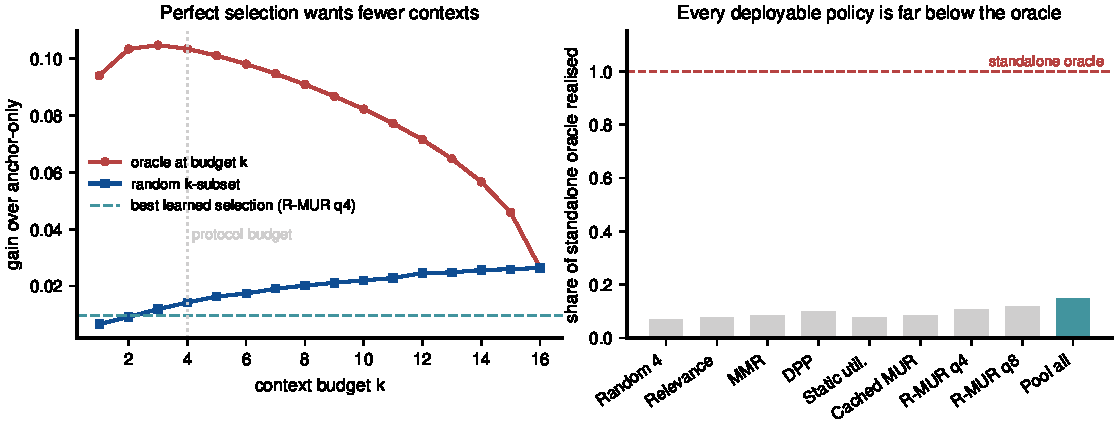
\includegraphics[width=0.98\textwidth]{figures/fig7_budget_gap.pdf}
  \caption{The identifiability gap under a strong predictor. Left: with true
  marginals the optimal budget is three contexts and the oracle decreases with
  every additional context, while random subsets improve monotonically, so the
  best deployable policy in the matrix is to include all sixteen candidates;
  the best learned selection is below random four. Right: share of the
  standalone-oracle gain realised by each deployable policy.}
  \label{fig:budget-gap}
\end{figure*}

\paragraph{The theory's central prediction, tested directly.}
\Cref{prop:suff} implies that the identifiable term is the fixed
predictor's own residual, so a \emph{stronger} predictor should leave \emph{less}
realizable value while the structural opportunity persists. We built a ladder of
experts on identical cells (eight targets, seed 101, same pools and episodes):
three spatio-temporal transformers of increasing capacity, a masked-mean MLP,
and the per-target ridge expert of the frozen protocol as an out-of-family
contrast. Strength is the anchor-only mean squared error on held-out windows;
realizable value is the learned router's share of the standalone-oracle gain.

\begin{table}[t]
 \centering
 \small
 \caption{Expert ladder on METR-LA (eight targets, seed 101). A stronger expert
 has a lower anchor-only MSE.}
 \label{tab:ladder}
 \begin{tabular}{lccccc}
  \toprule
  Expert & Anchor MSE & Standalone oracle & Sequential oracle & Learned gain & Realized share\\
  \midrule
  ridge (linear, out of family) & .3782 & $+.1535$ & $+.1687$ & $+.0313$ & $.198$\\
  transformer, 1 layer $d{=}32$ & .3721 & $+.0835$ & $+.0961$ & $+.0222$ & $.268$\\
  masked-mean MLP & .3625 & $+.1002$ & $+.1198$ & $+.0273$ & $.243$\\
  transformer, 2 layers $d{=}64$ & .3578 & $+.0923$ & $+.1044$ & $+.0168$ & $.177$\\
  transformer, 3 layers $d{=}128$ & .3562 & $+.0902$ & $+.1060$ & $+.0075$ & $.063$\\
  \bottomrule \end{tabular}
\end{table}

Within the neural family the prediction holds as a monotone dose--response: the
structural opportunity is flat ($+.084$ to $+.100$ standalone, $+.096$ to
$+.120$ sequential) while the realized share falls by a factor of $4.3$ and the
learned gain by a factor of $3.0$ as anchor-only error falls from $.372$ to
$.356$. Across the four neural rungs anchor-only error orders realized share
perfectly (Spearman $+1.0$), with a fitted slope of $10.5$ realized-share points
per unit anchor MSE: a $1\%$ anchor improvement corresponds to about $+.038$
share. A $4\%$ improvement in the expert removes three quarters of the value
that routing can realise.

The ridge rung is the informative exception, and it sharpens the theory rather
than contradicting it. The ridge expert has the \emph{worst} anchor-only error
($.3782$) yet the \emph{largest} structural opportunity ($+.1535$, because its
residual is highly systematic) and the largest absolute learned gain
($+.0313$); its realized \emph{share} ($.198$) is nonetheless below the weakest
transformer ($.268$), though above the two larger ones ($.177$ and $.063$),
because its denominator is larger. Including it, the rank correlation between
anchor error and realized share falls and the slope halves to $4.9$. Residual
magnitude is a sufficient statistic for realizable value only \emph{within} a fixed
hypothesis class; across families the inductive bias changes which candidates
are jointly improvable, so accuracy and residual geometry decouple. Anchor-only
accuracy is therefore not a sufficient statistic for identifiability across
architecture families: what matters is how much of the residual stays
predictable, and that quantity has to be measured, not inferred from a
leaderboard.

\subsection{Second Task Family: Demonstration Selection}
\label{sec:second-family}

To test whether the same decision object and the same method transfer outside
forecasting, we instantiate R-MUR on context-example selection for a frozen
in-context image classifier. Candidate contexts are labelled training images;
the anchor is a query image; the fixed predictor is a transformer that reads
the query embedding and the embeddings and labels of the selected
demonstrations; utility is the reduction of query-batch cross-entropy.
Embeddings come from a frozen CLIP ViT-L/14 encoder. Five public benchmarks are
used (CIFAR-10, CIFAR-100, SVHN, EuroSAT, DTD) with three seeds, $K=16$
candidates, budget four and 1{,}602 test episodes per benchmark. The router is
re-instantiated unchanged, including the seven-dimensional response summary,
now computed in class-logit space.

The predictor is genuinely in-context: mean accuracy rises from $0.966$ to
$0.983$ on CIFAR-10, $0.812$ to $0.997$ on CIFAR-100, $0.693$ to $0.996$ on
SVHN, $0.946$ to $0.986$ on EuroSAT and $0.728$ to $0.921$ on DTD when four
relevant demonstrations are added, and the farthest demonstrations are worse
than random ones. \Cref{tab:second-family} reports the gate. R-MUR beats both
response-free learned routers with a paired confidence interval above zero on
three of five benchmarks, and fails on CIFAR-100 and DTD, where a plain
nearest-neighbour relevance rule is already within a fraction of a percent of
the oracle.

\begin{table}[t]
 \centering
 \small
 \caption{Second task family. Mean cross-entropy reduction (nats) at $q=4$;
 $\Delta$ columns are paired contrasts against the two response-free learned
 routers. ``H-state'' is the sequential-over-standalone oracle gap.}
 \label{tab:second-family}
 \begin{tabular}{lccccc}
  \toprule
  Benchmark & R-MUR & Static & Cached & $\Delta$Static & $H_{\mathrm{state}}$\\
  \midrule
  CIFAR-10 & .0643 & .0482 & .0433 & $+.0160$ & .000\\
  CIFAR-100 & .5247 & .5769 & .5381 & $-0.0522$ & .000\\
  SVHN & .8809 & .7530 & .7688 & $+.1279$ & .000\\
  EuroSAT & .1294 & .1074 & .1125 & $+.0221$ & .000\\
  DTD & .3322 & .5981 & .6478 & $-0.2658$ & .000\\
  \bottomrule
 \end{tabular}
\end{table}

The second family also exposes a boundary condition of the framework. The
sequential and standalone oracles coincide to four decimals on all five
benchmarks ($H_{\mathrm{state}}\le 5\times10^{-4}$): because the candidate
pools contain no redundant demonstrations, selecting the best standalone
demonstrations is already optimal, and state-conditioning has nothing to
exploit. A nearest-neighbour relevance rule attains $99.4$--$99.9\%$ of the
oracle gain on every benchmark. The family therefore tests transfer of the
ranking machinery, not the state-conditioning mechanism that drives the
forecasting results, and it identifies the regime in which a simple baseline is
hard to beat: no redundancy among candidates and a predictor that is already
near-saturated with a handful of contexts. \Cref{fig:generality} (right) shows
the paired contrasts per benchmark.

A redundancy-structured variant tests the mechanism directly. We rebuilt the
candidate pools so that each contains four visual clusters with three
near-duplicate members each (measured within-cluster cosine similarity $.999$
for controlled copies against $.575$--$.838$ between clusters), and
pre-registered two predictions: redundant pools should create state-conditioning
headroom, and R-MUR should then beat both response-free learned routers. The
first prediction fails in substance. Redundancy is real --- a second
demonstration from the same cluster retains only $6.7$--$42\%$ of the first
member's marginal --- yet the sequential oracle exceeds the standalone oracle
by at most $0.09\%$ of its gain. The measured reason is that demonstration
utility is label-driven: replacing candidate features by noise costs only
$18\%$ of the first-member marginal and leaves later marginals unchanged,
whereas equalising labels flips every marginal negative. For this predictor the
utility is close to a function of the label multiset of the selected set, so no
pool geometry can make it state-conditioned.

We also iterated on the scoring head itself, in three steps, to test whether
the failure is one of functional form. Replacing the scalar head by the
theory-shaped bilinear score of \cref{eq:bilinear-head} improves the ranking of
the true marginal on four of five benchmarks (mean within-state Spearman $.375$
against $.156$; top-one agreement $.67$ against $.08$ on CIFAR-100) and gives
the largest pooled forced-budget contrast against Standalone Utility of the
three heads, $+.0605\;[-.0036,+.1343]$, with three of five per-benchmark
intervals above zero. The residual failure has a precise cause: the association
between response magnitude and marginal utility changes sign across benchmarks
($+.257$ on CIFAR-10, $-.590$ on CIFAR-100), while the identity's curvature term
has a fixed sign. Releasing that constraint --- a learned, signed, unconstrained
curvature coefficient --- confirms the diagnosis directly: the coefficient moves
from its $-.25$ initialisation to $+.14$, $+.13$, $+.11$ and $+.08$ on four of
the five benchmarks (significantly different from both $-.25$ and $0$,
$p<10^{-6}$), and is $\approx 0$ only on SVHN, exactly where the correlation
with the curvature term was weakest. But the gain does not follow. The signed
head's pooled contrast is $+.0528\;[-.0081,+.1236]$, it passes the
per-benchmark criterion on two of five rather than three, and it is uniformly no
better than the fixed-sign head; the extra unconstrained unit re-fits the same
ordering rather than improving it, because the learned first-order coefficient
already absorbs the ordering signal the curvature carries. Four head variants
--- scalar, curvature-corrected, bilinear and signed bilinear --- therefore
bracket the same result, which locates the ceiling in what the router can
observe rather than in how the score is parameterised.

The second prediction holds once the stopping rule is separated from the
ranking. The frozen rule stops when the predicted marginal becomes
non-positive, which truncates selection to $0.53$--$0.63$ of the budget on DTD
and fails the gate (pooled $\Delta$Static $-.162$). Forcing the budget to be
spent passes on five of five benchmarks in both pool environments, with pooled
$\Delta$Static $+.045\;[+.018,+.080]$ and $+.055\;[+.020,+.101]$ and
$\Delta$Cached $+.070$ and $+.108$, all with paired confidence intervals above
zero and passing under class-clustered intervals as well. The transferable part
of R-MUR is therefore its response-aware ranking; the threshold is a
calibration-dependent stopping device that should be fitted per family rather
than inherited.

\begin{figure*}[t]
  \centering
  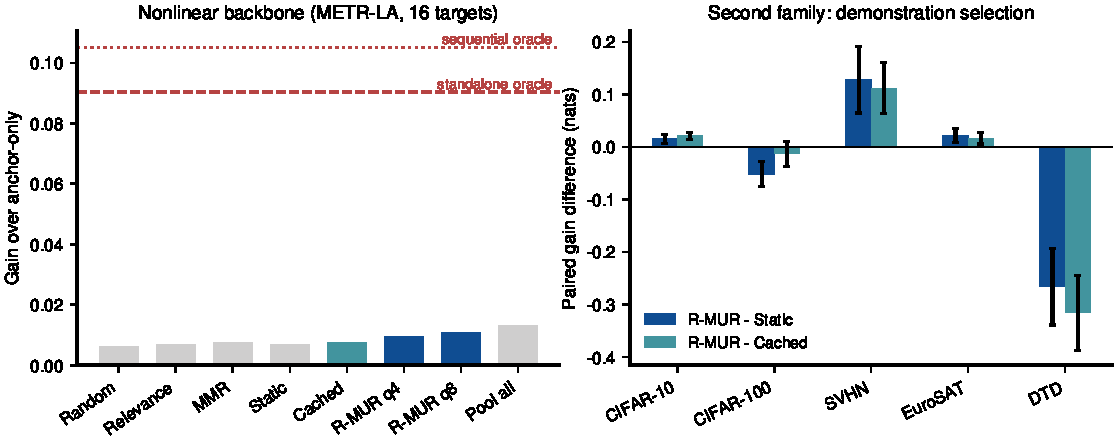
\includegraphics[width=0.98\textwidth]{figures/fig6_generality.pdf}
  \caption{Generality evidence. Left: with the subset-capable nonlinear
  backbone on METR-LA, every deployable policy remains far below the two oracle
  levels, and the learned response-free routers are indistinguishable from
  random selection. Right: in the second task family, R-MUR improves on both
  response-free learned routers on three of five benchmarks and degrades on the
  two where nearest-neighbour relevance is already within a fraction of a
  percent of the oracle. Bars are paired 95\% intervals.}
  \label{fig:generality}
\end{figure*}

% Gain--harm frontier values: KBS_MUR/results/derived/R204_harm_ladder_summary/summary.json
\subsection{What Determines Learned Routing Quality?}

Candidate-pool growth compresses the decision margin. In the controlled
scaling study, absolute utility error improves as $K$ increases, but the
standard deviation of true marginals falls faster. Normalized error rises from
.403 to .739, the positive top-two margin falls from .220 to .024, and the
median ratio of maximum candidate error to that margin rises from 1.17 to
3.40. Decision accuracy falls from .884 to .147, while one-step regret rises
from .018 to .067 at $K=16$ and remains elevated at .049 at $K=64$. Large
candidate pools therefore make the argmax decision harder even when pointwise
regression error improves in absolute units.

Predictor response determines whether marginal utility is observable. With
cached context features, the response-feature comparison reaches a Spearman
correlation of .164 and positive-utility AUC of .649. Adding compact
response summaries raises them to .391 and .834, improves top-1 accuracy from
.148 to .260, and reduces one-step regret from .0736 to .0569. Full forecast
trajectories add little beyond the compact summaries. These results motivate
the response-aware stage of R-MUR.

Finally, a calibration-derived stopping threshold traces a gain--harm
frontier. At harmful fraction .25 the uncalibrated router reaches a gain of
$.273$ with a negative-transfer rate of $.032$; calibration moves the same
policy to a gain of $.072$ with harm $.0001$, i.e.\ it buys an elevenfold
reduction in harm for three quarters of the gain. The same trade appears at
higher harmful fractions: at $.50$ the uncalibrated harm is $.085$ and at $.75$
it is $.227$, against calibrated harm of $.0006$ and $.0012$. The threshold
changes only the stopping decision; the candidate ranking remains the
response-aware score. Across all settings, R-MUR is greedy and targets
one-step decision quality under a context budget.
